\documentclass[11pt]{article}
\usepackage[margin=0.7in]{geometry}
\usepackage{amsmath,amssymb}
\usepackage{tikz}
\usetikzlibrary{positioning,arrows.meta}
\usepackage{enumitem}
\usepackage{hyperref}

\newcommand{\Con}{\operatorname{Con}}

\pagestyle{empty}

\begin{document}

\begin{center}
{\large\bfseries Congruence obstructions in exact predictive agents}\\[2pt]
{\small Revised project flow}\\[2pt]
{\footnotesize Classical predictive-state foundation in (1)--(4);
the contribution begins with transition-monoid descent in (5).}
\end{center}

\begin{center}
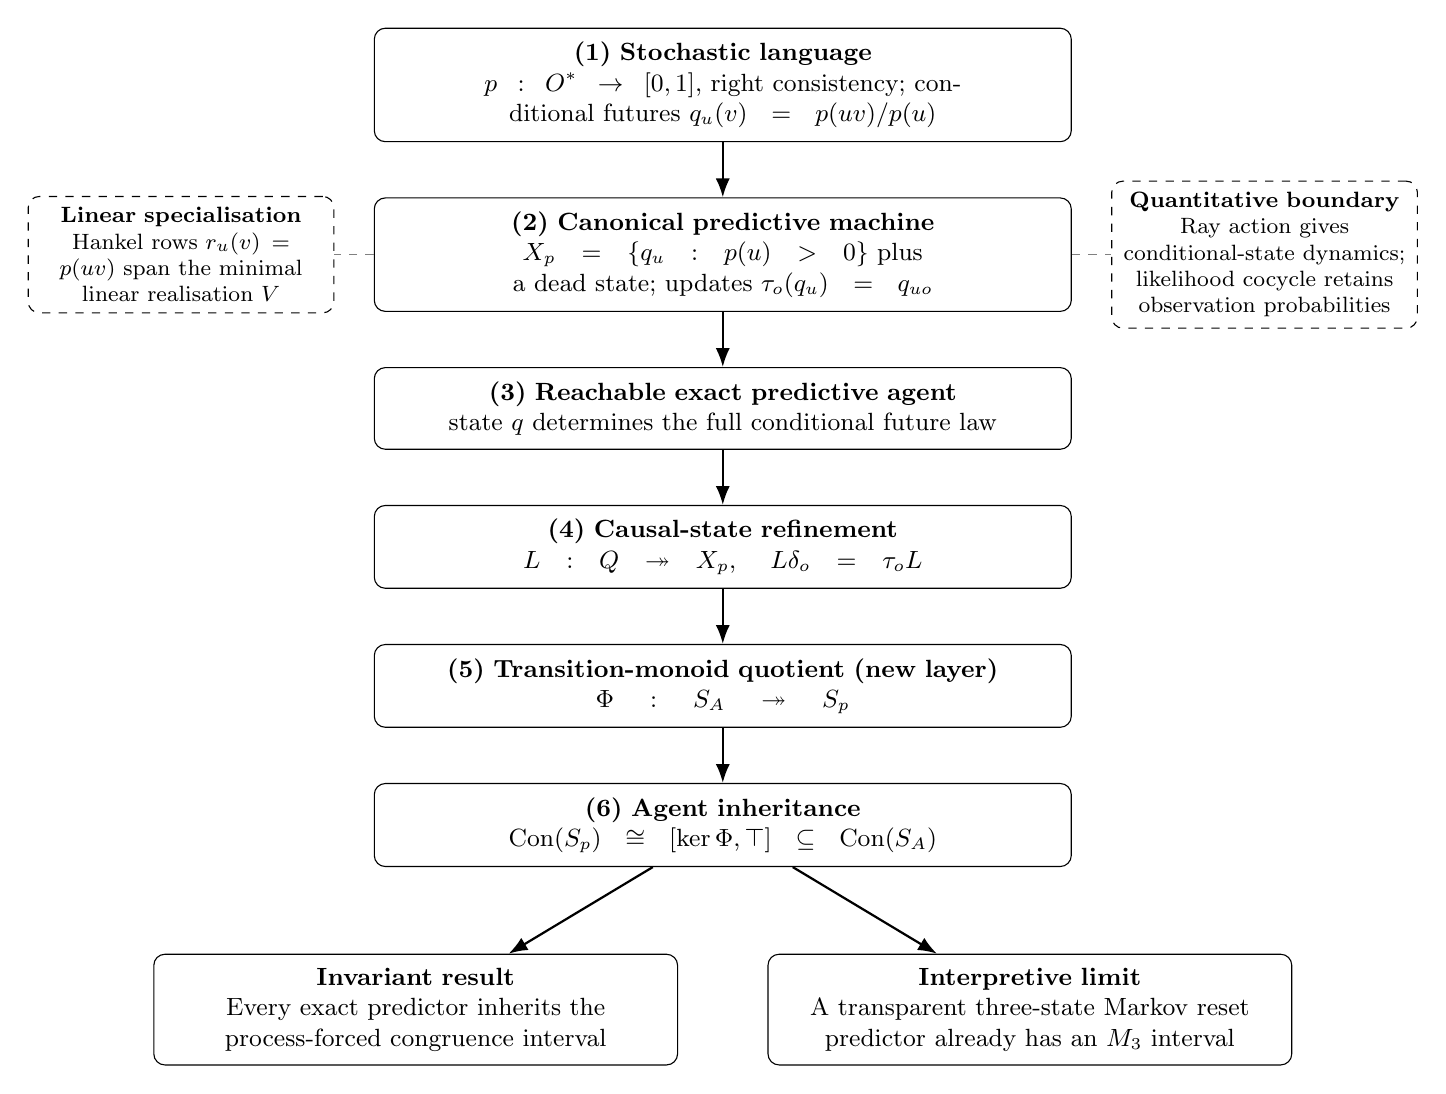
\begin{tikzpicture}[
  node distance=7mm,
  box/.style={draw,rounded corners,align=center,text width=8.5cm,
              inner sep=5pt,font=\small},
  result/.style={draw,rounded corners,align=center,text width=6.3cm,
                 inner sep=5pt,font=\small},
  side/.style={draw,dashed,rounded corners,align=center,text width=3.6cm,
               inner sep=4pt,font=\footnotesize},
  arr/.style={-{Latex[length=2.4mm]},thick},
  link/.style={dashed,gray}
]

\node[box] (p)
  {\textbf{(1) Stochastic language}\\
   $p:O^*\to[0,1]$, right consistency; conditional futures
   $q_u(v)=p(uv)/p(u)$};

\node[box,below=of p] (x)
  {\textbf{(2) Canonical predictive machine}\\
   $X_p=\{q_u:p(u)>0\}$ plus a dead state; updates
   $\tau_o(q_u)=q_{uo}$};

\node[box,below=of x] (a)
  {\textbf{(3) Reachable exact predictive agent}\\
   state $q$ determines the full conditional future law};

\node[box,below=of a] (quot)
  {\textbf{(4) Causal-state refinement}\\
   $L:Q\twoheadrightarrow X_p$, \quad
   $L\delta_o=\tau_oL$};

\node[box,below=of quot] (mon)
  {\textbf{(5) Transition-monoid quotient (new layer)}\\
   $\Phi:S_A\twoheadrightarrow S_p$};

\node[box,below=of mon] (con)
  {\textbf{(6) Agent inheritance}\\
   $\Con(S_p)\cong[\ker\Phi,\top]\subseteq\Con(S_A)$};

\node[result,below=11mm of con,xshift=-39mm] (positive)
  {\textbf{Invariant result}\\
   Every exact predictor inherits the process-forced congruence interval};

\node[result,below=11mm of con,xshift=39mm] (negative)
  {\textbf{Interpretive limit}\\
   A transparent three-state Markov reset predictor already has an $M_3$ interval};

\foreach \u/\v in {p/x,x/a,a/quot,quot/mon,mon/con}
  {\draw[arr] (\u)--(\v);}
\draw[arr] (con)--(positive);
\draw[arr] (con)--(negative);

\node[side,left=5mm of x] (linear)
  {\textbf{Linear specialisation}\\
   Hankel rows $r_u(v)=p(uv)$ span the minimal linear realisation $V$};

\node[side,right=5mm of x] (quant)
  {\textbf{Quantitative boundary}\\
   Ray action gives conditional-state dynamics; likelihood cocycle retains
   observation probabilities};

\draw[link] (x)--(linear);
\draw[link] (x)--(quant);

\end{tikzpicture}
\end{center}

\vspace{2mm}

\small
\begin{description}[leftmargin=1.6em,style=unboxed,itemsep=4pt]

\item[(1)] A stochastic language supplies consistent probabilities of finite
observation words.  Stationarity is optional and is stated separately.

\item[(2)] Positive-probability histories are identified exactly when they have
the same conditional distribution over every finite future.  Impossible
extensions go to one absorbing dead state.

\item[(3)] The agent theorem concerns reachable exact predictors.  It does not
assume that arbitrary hidden states of a neural network are linear, and it does
not follow from fixed-task controller optimality.

\item[(4)] Mapping an agent state to the future law it predicts is the
state-level refinement familiar from computational mechanics.  The controlled
counterpart is the $\varepsilon$-transducer, and the linear counterpart is
classical Hankel minimisation.

\item[(5)] Intertwining descends from states to generated transformations:
equal word transformations in the agent induce equal transformations on
canonical predictive states.

\item[(6)] Congruence correspondence makes the world's predictive transition
hierarchy an interval in the agent's hierarchy.  Redundancy may add structure
below the kernel but cannot remove the canonical interval.

\end{description}

\noindent\textbf{Novelty boundary.}
The contribution is the passage from the state intertwiner to the monoid
surjection, the inherited congruence interval and its $M_3/N_5$ witnesses, the
reset-monoid limitation below.  Canonical predictive states,
$\varepsilon$-transducers, Hankel minimisation, behavioural world-model
recovery, and predictive-memory necessity are prior work.

\medskip
\noindent\textbf{Main counterexample.}
For any first-order Markov chain on $n$ observations with full-support initial
distribution, full-support transition matrix, and distinct transition rows,
observing $i$ resets every feasible predictive state to the $i$th Markov row
and fixes the formal dead state.  Thus
\[
  S_p\cong R_n^1=\{1,c_1,\ldots,c_n\},\qquad c_ic_j=c_i.
\]
The congruences that fix $1$ form $\Pi_n$; for $n=3$ this is the interval
$\Pi_3\cong M_3$.  The predictor merely stores the latest observation, so
non-distributivity across this broad Markov class cannot certify entangled or
uninterpretable features.

\medskip
\noindent\textbf{Information boundary.}
The projective action of the minimal linear operators remembers the next
conditional state but forgets the probability of reaching it.  The pair
\[
  \left(T\cdot[r_u],\;
  \ell_T([r_u])=\frac{(Tr_u)(\varepsilon)}{r_u(\varepsilon)}\right)
\]
is faithful on the minimal Hankel space.  The projective quotient is therefore
called the \emph{conditional-state transition skeleton}, not the complete
stochastic process.

\medskip
\noindent\textbf{Controller result and boundary.}
A one-state controller can be optimal for a constant reward in a process with
many predictive states, so fixed-task optimality does not force a world model.
Richens et al.\ and Cifuentes obtain behavioural model recovery from sufficiently
general goal-conditioned policies, while Nayebi proves quantitative
predictive-memory necessity and no-aliasing results.  The behavioural/internal
distinction is therefore not claimed as new here.  Richens assumes deterministic
policies and full observation.  Cifuentes permits stochastic,
observation-history policies, but the partially observable theorem still uses
goals phrased in latent states; it does not recover arbitrary latent dynamics
from observation-only goals.

If behavioural recovery factors through recurrent controller state, or if a
complete zero-regret selection family forces recurrent memory to refine
predictive state on a transition-closed support, then
\[
  M(h)=M(h')\Longrightarrow\eta(h)=\eta(h'),
  \qquad
  L\delta_{a,o}=\tau_{a,o}L,\qquad
  S_C\twoheadrightarrow S_{\mathcal I},
\]
and the controlled predictive congruence lattice occurs as an interval in the
controller's.  At finite regret, Nayebi's result only bounds the evaluated mass
of predictive aliases; it does not produce an exact congruence interval.

\medskip
\noindent\textbf{Extension.}
Combine Cifuentes's common-support residual metric and predictive-state
separation theorem with monoid descent to study robust persistence of finite
$M_3/N_5$ witnesses.

\end{document}
